\section{Introduzione ai LLM}
I \emph{Language Model} (LM) sono modelli linguistici, basati sul \emph{machine learning}, che vengono addestrati su quantit\`a enormi di dati e per questo vengono chiamati \emph{Large Languge Model}, essi generano ed elaborano testo in linguaggio naturale. \\
Negli ultimi tempi il campo del \emph{Natural Language Processing} (NLP) si \`e evoluto con una rapidit\`a molto elevata, questo grazie a tutte le ricerche fatte e i progressi ottenuti in ambito scientifico e tecnologico. 
Il NLP \`e un'area di studio che fa convergere informatica, intelligenza artificiale e linguistica, l'obiettivo \`e quello di far elaborare a una macchina del testo in linguaggio naturale, "capirne" il significato e coglierne le sfumature emotive \cite{blaise2022llmunderstandus}.\\
In passato i LLM erano costruiti attraverso le \emph{Recurrent Neural Network}, (RNN) pi\`u precisamente mediante un'architettura nota come \emph{Long short-term memory} (LSTM) il cui obiettivo \`e quello di ridurre il problema della scomparsa del gradiente presente nelle RNN.
Al giorno d'oggi lo stato dell'arte \`e diverso, infatti troviamo che i modelli pi\`u performanti sono quelli basati sui \emph{Transformer} \cite{vaswani2023attentionneed}.

\section{Transformer}
Un \emph{Transformer}, di norma, \`e composto da un \emph{encoder} e un \emph{decoder}, figura \ref{fig:architetturaTransformer}, entrambe le parti sono composte da \emph{layer} fortemente connessi.
Esso prende in input del testo in linguaggio naturale e lo rielabora trasformandolo in una rappresentazione numerica composta da sequenze di token.
\begin{figure}[H]
    \centering
    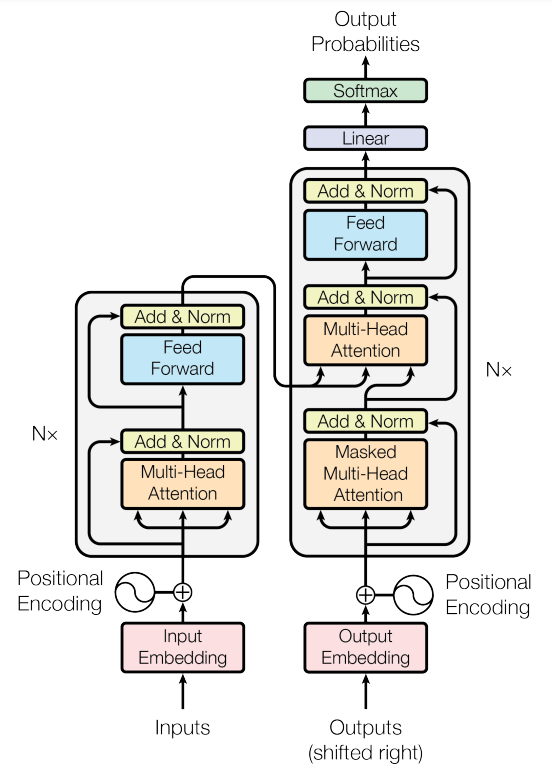
\includegraphics[width=0.4\textwidth]{media/1-introduzioneLLM/thetransformerarchitecture.png}
    \caption{L'architettura di un \emph{Transformer}. Immagine presa da \cite{vaswani2023attentionneed}.}
    \label{fig:architetturaTransformer}
\end{figure}

I \emph{Transformer} basano la loro forza sulla \emph{Self-Attention}, questo \`e un meccanismo che permette di creare collegamenti globali tra l'input e l'output, ci\`o ha permesso di liberarsi dall'uso delle \emph{recurrent unit} presenti nelle RNN. Queste unit\`a fungevano da memoria il quale valore riceveva un aggiornamento per ogni passo eseguito durante l'apprendimento della rete, questa modalit\`a di aggiornamento dei valori \`e fortemente inefficiente rispetto alla tecnica della \emph{Self-Attention}.

\subsection{Funzionamento e Self-Attention}
La \emph{Self-Attention} \`e il meccanismo chiave per il funzionamento dell'architettura \emph{Transformer}. Questa tecnologia consente al modello di considerare ed esaminare contemporaneamente l'intera sequenza di token ricevuta in input, contrariamente a quanto fanno le RNN, che elaborano i dati sequenzialmente.
Inoltre \emph{Self-Attention} riesce ad attribuire a ogni token un valore che rappresenta la rilevanza di questo all'interno dell'input.\\
Quando viene dato al \emph{Transformer} un input, come ad esempio una frase in linguaggio naturale, questo lo prende e lo rappresenta come una sequenza di numeri. Quest'operazione si chiama \emph{embedding}, ed \`e la pratica di associare ad ogni token un numero e creare un vettore di numeri, cosicch\'e il modello riesca a lavorare effettivamente su dei numeri, interpretabili correttamente dalla rete, e non su del testo.\\
A questo punto possiamo calcolare l'\emph{attention} attraverso un prodotto scalare come nella figura \ref{fig:scaledDotProductAttention}:
\begin{figure}[H]
    \centering
    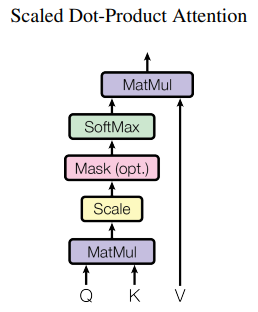
\includegraphics[width=0.4\textwidth]{media/1-introduzioneLLM/scaledDotProductAttention.png}
    \caption{Calcolo dell'\emph{attention} attraverso il prodotto scalare. Immagine presa da \cite{vaswani2023attentionneed}.}
    \label{fig:scaledDotProductAttention}
\end{figure}

\[\text{Attention}(Q,K,V)=\text{softmax}(\frac{QK^T}{\sqrt{d_k}})V\]
dove \(Q\) \`e la matrice delle query da elaborare,
\(K\) \`e la matrice delle chiavi e \(V\) e la matrice dei valori.\\
Un grande vantaggio che implementano i \emph{Transformer} \`e quello della parallelizzazione del calcolo dell'\emph{attention}, infatti attraverso la \emph{Multi-Head Attention} \`e possibile eseguire in parallelo pi\`u istanze della funzione \textsc{Attention} e concatenarne i risultati, come nella figura \ref{fig:multiHeadAttention}. Ci\`o rende i \emph{Transformer} incredibilmente pi\`u efficienti rispetto alle RNN.
\begin{figure}[H]
    \centering
    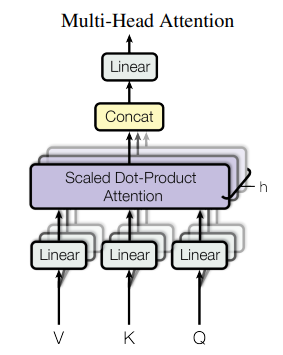
\includegraphics[width=0.4\textwidth]{media/1-introduzioneLLM/multiHeadAttention.png}
    \caption{\emph{Multi-Head Attention}. Immagine presa da \cite{vaswani2023attentionneed}.}
    \label{fig:multiHeadAttention}
\end{figure}

\section{A Che Cosa Servono i LLM}
Lo stato dell'arte dei LLM include diversi modelli, alcuni sono \emph{open source} altri invece no.
Tra i modelli pi\`u popolari e performanti troviamo:
\begin{itemize}
    \item ChatGPT 4o \cite{openaihellogpt4o}
    \item LLaMa 3 \cite{dubey2024llama3herdmodels}
    \item Mistral Large 2 \cite{mistralaimistrallarge2}
    \item Claude 3.5 Sonnet \cite{anthropicclaude35sonnet}
\end{itemize}
Questi modelli sono altamente potenti e in grado di elaborare e generare testo in linguaggio naturale, molti sono anche multi-modali: ovvero riescono a ricevere degli input diversi dal semplice linguaggio naturale, come ad esempio immagini, video oppure altri tipi di documenti.
Il grande punto di forza dei \emph{Large Language Model} risiede nel cogliere le varie sfaccettature che rendono unico ogni tipo di input, capirne il contesto ed elaborare una risposta coerente con le richieste.
Tutto ci\`o rende fortemente utili i LLM, infatti nell'ultimo periodo hanno raggiunto lo status di assistenti virtuali i quali riescono a completare con successo quasi tutte le richieste di un utente medio che si interfaccia a essi. Esistono per\`o delle tecniche di \emph{fooling} che permettono di compromettere l'affidabilit\`a e la sicurezza di questi modelli, anche dei pi\`u avanzati. Bisogna perci\`o sapere come usarli e i proprietari di questi modelli devono essere in grado di difendersi dai pericoli che ne derivano per loro e per i loro clienti.
